\documentclass{beamer}
\IfFileExists{beamerthemeUASLP1.sty}{
    \usetheme{UASLP1}
}{
    \usetheme{Madrid}
    \usecolortheme{seahorse}
}

\usepackage[utf8]{inputenc}
\usepackage[T1]{fontenc}
\usepackage{helvet}
\usepackage{listings}
\usepackage{xcolor}
\usepackage{tikz}
\usepackage{hyperref}

\lstset{
    basicstyle=\ttfamily\footnotesize,
    keywordstyle=\color{blue},
    commentstyle=\color{gray},
    stringstyle=\color{red},
    showstringspaces=false,
    breaklines=true,
    frame=single,
    numbers=left,
    numberstyle=\tiny\color{gray}
}

\title{Course 2: LoRa Basics Modem}
\subtitle{LBM Architecture \& Integration}
\author{Dr. ABDELMALEK OMAR}
\date{\today}
\institute{USP Zephyr Training Series\\Copyright \copyright{} 2025 Dr. ABDELMALEK OMAR}

\begin{document}

\begin{frame}[plain,t]
\titlepage
\end{frame}

\begin{frame}
\frametitle{Course Overview}
\framesubtitle{What You'll Learn}
\begin{itemize}
    \item LoRa Basics Modem Architecture
    \begin{itemize}
        \item Event-driven programming model
        \item Modem API and services
        \item Stack lifecycle management
    \end{itemize}
    \item Advanced Features
    \begin{itemize}
        \item Low power optimization
        \item GNSS geolocation
        \item LoRaWAN Relay
    \end{itemize}
    \item Hands-On Labs (5 labs)
    \begin{itemize}
        \item Lab 2.1: Build and run periodical uplink
        \item Lab 2.2: Custom event handler
        \item Lab 2.3: Low power configuration
        \item Lab 2.4: GNSS geolocation
        \item Lab 2.5: Relay TX configuration
    \end{itemize}
\end{itemize}
\end{frame}

\section{LBM Architecture}

\begin{frame}
\frametitle{What is LoRa Basics Modem?}
\framesubtitle{Semtech's Official LoRaWAN Stack}

\begin{block}{Definition}
LoRa Basics Modem (LBM) is Semtech's production-ready LoRaWAN stack implementing the complete MAC layer protocol.
\end{block}

\begin{columns}[T]
\column{0.5\textwidth}
\textbf{Features:}
\begin{itemize}
    \item LoRaWAN 1.0.4 certified
    \item Event-driven architecture
    \item Low power optimized
    \item Built-in services:
    \begin{itemize}
        \item GNSS scanning
        \item LoRaWAN Relay
        \item FUOTA support
        \item Class A/B/C
    \end{itemize}
\end{itemize}

\column{0.5\textwidth}
\textbf{Version Info:}
\begin{itemize}
    \item Current: v4.9.0
    \item License: BSD-3-Clause
    \item Maintained by Semtech
    \item Used in production
\end{itemize}

\vspace{1em}

\textbf{USP Integration:}
\begin{itemize}
    \item Zephyr RTOS port
    \item Device tree config
    \item West workspace
\end{itemize}
\end{columns}
\end{frame}

\begin{frame}
\frametitle{LBM Architecture}
\framesubtitle{Software Stack Layers}

\begin{center}
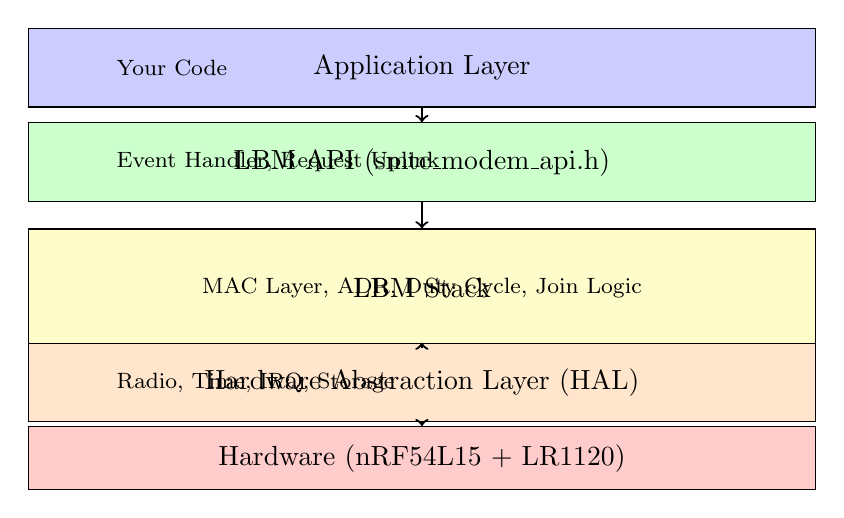
\begin{tikzpicture}[scale=0.8]
    % Application Layer
    \node[draw, rectangle, minimum width=10cm, minimum height=1cm, fill=blue!20] (app) at (0,5) {Application Layer};
    \node[right] at (-5,5) {\footnotesize Your Code};

    % LBM API
    \node[draw, rectangle, minimum width=10cm, minimum height=1cm, fill=green!20] (api) at (0,3.5) {LBM API (smtc\_modem\_api.h)};
    \node[right] at (-5,3.5) {\footnotesize Event Handler, Request Uplink};

    % LBM Stack
    \node[draw, rectangle, minimum width=10cm, minimum height=1.5cm, fill=yellow!20] (stack) at (0,1.5) {LBM Stack};
    \node at (0,1.5) {\footnotesize MAC Layer, ADR, Duty Cycle, Join Logic};

    % HAL Layer
    \node[draw, rectangle, minimum width=10cm, minimum height=1cm, fill=orange!20] (hal) at (0,0) {Hardware Abstraction Layer (HAL)};
    \node[right] at (-5,0) {\footnotesize Radio, Time, IRQ, Storage};

    % Hardware
    \node[draw, rectangle, minimum width=10cm, minimum height=0.8cm, fill=red!20] (hw) at (0,-1.2) {Hardware (nRF54L15 + LR1120)};

    % Arrows
    \draw[->, thick] (app) -- (api);
    \draw[->, thick] (api) -- (stack);
    \draw[->, thick] (stack) -- (hal);
    \draw[->, thick] (hal) -- (hw);
\end{tikzpicture}
\end{center}

\textbf{Key Point:} Application code only interacts with LBM API, not hardware directly.
\end{frame}

\begin{frame}[fragile]
\frametitle{Event-Driven Programming}
\framesubtitle{How LBM Communicates with Application}

\begin{block}{Event Loop Pattern}
LBM uses events to notify the application of state changes and incoming data.
\end{block}

\begin{lstlisting}[language=C, basicstyle=\tiny\ttfamily]
void event_handler(void)
{
    smtc_modem_event_t event;
    uint8_t pending_count;

    while (smtc_modem_get_event(&event, &pending_count) == SMTC_MODEM_RC_OK) {
        switch (event.event_type) {
        case SMTC_MODEM_EVENT_JOINED:
            LOG_INF("Network joined!");
            break;

        case SMTC_MODEM_EVENT_TXDONE:
            LOG_INF("TX done: %u", event.event_data.txdone.status);
            break;

        case SMTC_MODEM_EVENT_DOWNDATA:
            LOG_INF("Downlink received");
            handle_downlink(&event);
            break;
        }
    }
}

int main(void) {
    smtc_modem_init(event_handler);  // Register callback
    while(1) {
        smtc_modem_run_engine();      // Process events
        k_msleep(100);
    }
}
\end{lstlisting}
\end{frame}

\begin{frame}
\frametitle{LBM Event Types}
\framesubtitle{Complete Event Reference}

\begin{table}
\tiny
\begin{tabular}{|l|p{6cm}|}
\hline
\textbf{Event} & \textbf{Description} \\
\hline
JOINED & Network join successful \\
JOINFAIL & Join attempt failed \\
TXDONE & Uplink transmission complete \\
DOWNDATA & Downlink data received \\
LINK\_CHECK & Link check result available \\
CLASS\_B\_STATUS & Class B beacon status \\
ALARM & Alarm timer expired \\
GNSS\_SCAN\_DONE & GNSS scan completed \\
RELAY\_TX\_SYNC & Relay TX synchronized \\
FUOTA & Firmware update event \\
\hline
\end{tabular}
\end{table}

\vspace{1em}

\textbf{Best Practice:} Process events in a dedicated thread to avoid blocking modem engine.
\end{frame}

\begin{frame}[fragile]
\frametitle{LBM API Basics}
\framesubtitle{Common Operations}

\textbf{Initialization:}
\begin{lstlisting}[language=C, basicstyle=\tiny\ttfamily]
smtc_modem_init(event_handler);
smtc_modem_set_region(STACK_ID, SMTC_MODEM_REGION_EU_868);
\end{lstlisting}

\textbf{Join Network:}
\begin{lstlisting}[language=C, basicstyle=\tiny\ttfamily]
smtc_modem_join_network(STACK_ID);
\end{lstlisting}

\textbf{Send Uplink:}
\begin{lstlisting}[language=C, basicstyle=\tiny\ttfamily]
uint8_t payload[] = {0x01, 0x02, 0x03};
smtc_modem_request_uplink(STACK_ID,
                          2,      // Port
                          false,  // Unconfirmed
                          payload,
                          3);     // Length
\end{lstlisting}

\textbf{Get Status:}
\begin{lstlisting}[language=C, basicstyle=\tiny\ttfamily]
smtc_modem_status_mask_t status;
smtc_modem_get_status(STACK_ID, &status);
if (status & SMTC_MODEM_STATUS_JOINED) {
    LOG_INF("Connected to network");
}
\end{lstlisting}
\end{frame}

\section{Low Power Optimization}

\begin{frame}
\frametitle{Power Consumption Breakdown}
\framesubtitle{Where Does Power Go?}

\begin{table}
\small
\begin{tabular}{|l|c|c|c|}
\hline
\textbf{State} & \textbf{Current} & \textbf{Duration} & \textbf{Energy} \\
\hline
Sleep & 25 µA & 95\% & 0.57 mAh/day \\
TX (SF7, +14dBm) & 100 mA & 41 ms × 24 & 0.027 mAh/day \\
RX1 Window & 15 mA & 100 ms × 24 & 0.010 mAh/day \\
RX2 Window & 15 mA & 100 ms × 24 & 0.010 mAh/day \\
\hline
\multicolumn{3}{|r|}{\textbf{Total (60s interval):}} & \textbf{0.62 mAh/day} \\
\hline
\end{tabular}
\end{table}

\textbf{Battery Life Calculation (2000 mAh):}
\[
\text{Life} = \frac{2000 \text{ mAh} \times 0.7}{0.62 \text{ mAh/day}} = 2258 \text{ days} \approx 6.2 \text{ years}
\]

\begin{alertblock}{Key Insight}
Sleep current dominates for long-lived sensors! Optimize sleep mode first.
\end{alertblock}
\end{frame}

\begin{frame}
\frametitle{Low Power Strategies}
\framesubtitle{Extend Battery Life}

\textbf{1. Increase Uplink Interval}
\begin{itemize}
    \item 60s → 300s (5min): 5× battery life improvement
    \item Consider application requirements
\end{itemize}

\textbf{2. Optimize Spreading Factor}
\begin{itemize}
    \item SF12: 991 ms ToA, but better sensitivity
    \item SF7: 41 ms ToA, but requires good link
    \item Use ADR to find optimal balance
\end{itemize}

\textbf{3. Reduce Payload Size}
\begin{itemize}
    \item Fewer bytes = shorter ToA
    \item Use efficient encoding (binary, not JSON!)
\end{itemize}

\textbf{4. Disable Unnecessary Features}
\begin{itemize}
    \item No LED blinking
    \item Disable UART console in production
    \item Use confirmed uplinks sparingly
\end{itemize}

\textbf{5. Hardware Optimization}
\begin{itemize}
    \item Enable Zephyr power management
    \item Put external sensors to sleep
    \item Use external RTC for long sleep
\end{itemize}
\end{frame}

\section{GNSS Geolocation}

\begin{frame}
\frametitle{GNSS with LR1120/LR1121}
\framesubtitle{Satellite-Based Positioning}

\begin{columns}[T]
\column{0.5\textwidth}
\textbf{How It Works:}
\begin{enumerate}
    \item LR1120 scans for GPS/BeiDou satellites
    \item Generates NAV (navigation) message
    \item Send NAV to LoRa Cloud via LoRaWAN
    \item Cloud solver returns position
\end{enumerate}

\vspace{1em}

\textbf{Advantages:}
\begin{itemize}
    \item No dedicated GPS receiver needed
    \item Passive scanning (no TX)
    \item Works with obstructed view
    \item Low power (< 500 mAs per scan)
\end{itemize}

\column{0.5\textwidth}
\textbf{Accuracy:}
\begin{itemize}
    \item Outdoor, clear sky: 10-30m
    \item Near window: 30-100m
    \item Indoor: May fail or >100m
\end{itemize}

\vspace{1em}

\textbf{Scan Modes:}
\begin{description}
    \item[STATIC:] Device not moving, longer scan
    \item[MOBILE:] Device moving, shorter scan
\end{description}

\vspace{1em}

\textbf{Time to Fix:}
\begin{itemize}
    \item With assistance: 30-60s
    \item Cold start: 2-5 min
\end{itemize}
\end{columns}
\end{frame}

\begin{frame}[fragile]
\frametitle{GNSS Implementation}
\framesubtitle{Code Example}

\begin{lstlisting}[language=C, basicstyle=\tiny\ttfamily]
// Configure GNSS
smtc_modem_gnss_set_constellation(STACK_ID,
    SMTC_MODEM_GNSS_CONSTELLATION_GPS_BEIDOU);

// Set assistance position (approximate location)
smtc_modem_gnss_assistance_position_t assist = {
    .latitude = 37.7749,
    .longitude = -122.4194,
};
smtc_modem_gnss_set_assistance_position(STACK_ID, &assist);

// Start scan
smtc_modem_gnss_scan(STACK_ID, SMTC_MODEM_GNSS_MODE_STATIC);

// In event handler:
case SMTC_MODEM_EVENT_GNSS_SCAN_DONE:
    uint8_t nav_message[255];
    uint16_t nav_size;

    smtc_modem_gnss_get_event_data_scan_done(STACK_ID,
                                             nav_message,
                                             &nav_size);

    // Send NAV to cloud solver
    smtc_modem_request_uplink(STACK_ID, 192, false,
                              nav_message, nav_size);
    break;
\end{lstlisting}
\end{frame}

\section{LoRaWAN Relay}

\begin{frame}
\frametitle{LoRaWAN Relay}
\framesubtitle{Extend Network Coverage}

\begin{center}
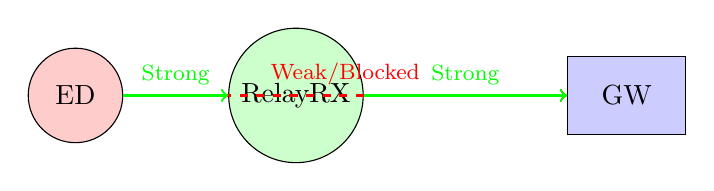
\begin{tikzpicture}[scale=0.7]
    % End Device (weak signal to GW)
    \node[draw, circle, minimum size=1.2cm, fill=red!20] (ed) at (0,0) {ED};

    % Gateway (far away)
    \node[draw, rectangle, minimum width=1.5cm, minimum height=1cm, fill=blue!20] (gw) at (10,0) {GW};

    % Relay RX (good signal to both)
    \node[draw, circle, minimum size=1.2cm, fill=green!20] (relay) at (4,0) {Relay\\RX};

    % Weak direct path
    \draw[->, dashed, red, thick] (ed) -- (gw) node[midway, above] {\footnotesize Weak/Blocked};

    % Strong relay path
    \draw[->, green, thick] (ed) -- (relay) node[midway, above] {\footnotesize Strong};
    \draw[->, green, thick] (relay) -- (gw) node[midway, above] {\footnotesize Strong};
\end{tikzpicture}
\end{center}

\textbf{Use Cases:}
\begin{itemize}
    \item Indoor sensors with outdoor gateway
    \item Extending range in difficult terrain
    \item Connecting devices in basements/underground
\end{itemize}

\textbf{Types:}
\begin{description}
    \item[Relay RX:] Mains-powered, Class C, forwards uplinks
    \item[Relay TX:] Battery-powered end device, relayed by RX
\end{description}
\end{frame}

\begin{frame}[fragile]
\frametitle{Relay TX Configuration}
\framesubtitle{Enable Relay for End Device}

\begin{lstlisting}[language=C, basicstyle=\tiny\ttfamily]
// After join, enable Relay TX
smtc_modem_relay_tx_enable(STACK_ID,
    SMTC_MODEM_RELAY_TX_ACTIVATION_MODE_ENABLE);

// In event handler:
case SMTC_MODEM_EVENT_RELAY_TX_SYNC:
    LOG_INF("Synchronized with Relay RX");
    LOG_INF("  Relay DevAddr: 0x%08X",
            event.event_data.relay_tx_sync.relay_dev_addr);
    break;

case SMTC_MODEM_EVENT_TXDONE:
    // Check if uplink was relayed
    smtc_modem_relay_tx_uplink_info_t info;
    smtc_modem_relay_tx_get_last_uplink_info(STACK_ID, &info);

    if (info.was_relayed) {
        LOG_INF("Uplink was RELAYED");
        LOG_INF("  Via: 0x%08X", info.relay_dev_addr);
    } else {
        LOG_INF("Direct uplink (not relayed)");
    }
    break;
\end{lstlisting}

\textbf{Power Benefit:} Relay TX can use lower TX power, saving battery!
\end{frame}

\section{Hands-On Labs}

\begin{frame}
\frametitle{Lab 2.1: Build and Run Periodical Uplink}
\framesubtitle{Your First LBM Application}

\textbf{Objective:} Build, flash, and run the LBM periodical uplink sample.

\textbf{Steps:}
\begin{enumerate}
    \item Configure credentials in device tree overlay
    \item Build: \texttt{west build -p -b xiao\_nrf54l15\_nrf54l15\_cpuapp \textbackslash\\
          --shield semtech\_lr1120mb1dis samples/usp/lbm/periodical\_uplink}
    \item Flash: \texttt{west flash}
    \item Monitor: \texttt{minicom -D /dev/ttyACM0 -b 115200}
    \item Verify on network server (TTN/ChirpStack)
\end{enumerate}

\textbf{Expected Output:}
\begin{itemize}
    \item Join successful within 10 seconds
    \item Uplinks every 60 seconds
    \item RSSI/SNR values logged
\end{itemize}

\textbf{Deliverables:}
\begin{itemize}
    \item Serial log showing join + 10 uplinks
    \item Network server screenshot
\end{itemize}
\end{frame}

\begin{frame}[fragile]
\frametitle{Lab 2.2: Custom Event Handler}
\framesubtitle{Advanced Event Processing}

\textbf{Objective:} Implement custom logic to track success rate and detect failures.

\textbf{Features to Implement:}
\begin{enumerate}
    \item Track uplink success rate (confirmed vs total)
    \item Alert if 3 consecutive failures
    \item Log RSSI/SNR of downlinks
    \item Automatic ADR profile switching based on link quality
\end{enumerate}

\textbf{Example Alert Logic:}
\begin{lstlisting}[language=C, basicstyle=\tiny\ttfamily]
static uint8_t consecutive_failures = 0;

case SMTC_MODEM_EVENT_TXDONE:
    if (event.event_data.txdone.status == SMTC_MODEM_EVENT_TXDONE_CONFIRMED) {
        consecutive_failures = 0;
    } else {
        consecutive_failures++;
        if (consecutive_failures >= 3) {
            send_alert_uplink();  // Notify server
        }
    }
    break;
\end{lstlisting}

\textbf{Deliverables:}
\begin{itemize}
    \item Complete source code with tracking
    \item Test report showing failure detection
    \item Success rate calculation over 50 uplinks
\end{itemize}
\end{frame}

\begin{frame}
\frametitle{Lab 2.3: Low Power Configuration}
\framesubtitle{Optimize for Battery Life}

\textbf{Objective:} Configure LBM for minimum power consumption.

\textbf{Tasks:}
\begin{enumerate}
    \item Build with low power config: \texttt{prj\_lowpower.conf}
    \item Measure power with Nordic Power Profiler Kit II
    \item Compare different uplink intervals (60s, 300s, 900s)
    \item Calculate battery life for each configuration
\end{enumerate}

\textbf{Measurements to Take:}
\begin{itemize}
    \item Sleep current (should be < 30 µA)
    \item TX current and duration
    \item RX window current and duration
    \item Average current per uplink cycle
\end{itemize}

\textbf{Expected Results:}
\begin{table}
\footnotesize
\begin{tabular}{|l|c|c|}
\hline
\textbf{Interval} & \textbf{Avg Current} & \textbf{Battery Life} \\
\hline
60 seconds & 500 µA & 166 days \\
300 seconds & 100 µA & 833 days \\
900 seconds & 45 µA & 1,851 days \\
\hline
\end{tabular}
\end{table}
\end{frame}

\begin{frame}
\frametitle{Lab 2.4: GNSS Geolocation}
\framesubtitle{Satellite-Based Positioning}

\textbf{Objective:} Implement GNSS scanning and solve position with LoRa Cloud.

\textbf{Prerequisites:}
\begin{itemize}
    \item LR1120 or LR1121 radio (has GNSS capability)
    \item Clear view of sky (outdoors or near window)
    \item LoRa Cloud account with MGMS token
\end{itemize}

\textbf{Steps:}
\begin{enumerate}
    \item Configure GNSS constellation (GPS + BeiDou)
    \item Set assistance position (approximate location)
    \item Start GNSS scan after join
    \item Send NAV message to LoRa Cloud
    \item Receive solved position as downlink
    \item Visualize on map (Python script provided)
\end{enumerate}

\textbf{Deliverables:}
\begin{itemize}
    \item Serial log showing NAV message and solved position
    \item HTML map with position marker
    \item Accuracy analysis (compare to ground truth)
\end{itemize}
\end{frame}

\begin{frame}
\frametitle{Lab 2.5: Relay TX Configuration}
\framesubtitle{Extended Range with Relay}

\textbf{Objective:} Configure device as Relay TX (relayed end-device).

\textbf{Prerequisites:}
\begin{itemize}
    \item Two devices: one Relay TX (this lab), one Relay RX
    \item Network server supporting LoRaWAN Relay
\end{itemize}

\textbf{Setup:}
\begin{enumerate}
    \item Configure and deploy Relay RX near gateway
    \item Configure this device as Relay TX
    \item Enable Relay TX mode after join
    \item Verify uplinks are relayed (check metadata)
    \item Measure power savings from reduced TX power
\end{enumerate}

\textbf{Verification:}
\begin{itemize}
    \item Serial log shows "Relay TX synchronized"
    \item Uplink events indicate "was relayed"
    \item Network server shows relay metadata
\end{itemize}

\textbf{Deliverables:}
\begin{itemize}
    \item Relay TX code
    \item Network server logs showing relayed uplinks
    \item Power comparison (direct vs relayed)
\end{itemize}
\end{frame}

\begin{frame}
\frametitle{Course 2 Summary}
\framesubtitle{Key Takeaways}

\textbf{You've Learned:}
\begin{itemize}
    \item LBM Architecture: Event-driven, modular, production-ready
    \item Event Processing: How to handle JOIN, TXDONE, DOWNDATA events
    \item Low Power: Optimize sleep, interval, SF, payload for max battery life
    \item GNSS: Satellite positioning without dedicated GPS receiver
    \item Relay: Extend coverage using relay RX/TX devices
    \item Practical Skills: Build, optimize, and deploy LBM applications
\end{itemize}

\vspace{1em}

\textbf{Best Practices:}
\begin{itemize}
    \item Always use event-driven pattern (don't poll!)
    \item Test power consumption early in development
    \item Use ADR for optimal SF selection
    \item Consider Relay for indoor/difficult deployments
\end{itemize}

\vspace{1em}

\textbf{Next Course:} Course 3 - USP RAC Architecture (Multiprotocol)
\end{frame}

\begin{frame}[plain]
\centering
\Huge Thank You!

\vspace{2em}

\large Questions?

\vspace{2em}

\normalsize

\end{frame}

\end{document}
